\documentclass[aspectratio=169]{beamer}
\usetheme{Madrid}
\usecolortheme{default}
\setbeamertemplate{navigation symbols}{}
\setbeamertemplate{footline}[frame number]

% Pacotes necessários
\usepackage[utf8]{inputenc}
\usepackage[T1]{fontenc}
\usepackage[portuguese]{babel}
\usepackage{amsmath,amssymb,amsfonts}
\usepackage{graphicx}
\usepackage{booktabs}
\usepackage{multirow}
\usepackage{array}
\usepackage{siunitx}
\usepackage{acronym}
\usepackage{tabularx}

% Configurações de cores
\definecolor{myblue}{RGB}{31,119,180}
\definecolor{myred}{RGB}{214,39,40}
\definecolor{mygreen}{RGB}{44,160,44}

% Título da apresentação
\title{Efeitos do Lobbying na Atividade Parlamentar: \\ Modelagem PPML e Análise Causal}
\subtitle{Evidências do Parlamento Europeu (2019-2024)}
\author{Análise Empírica}
\institute{Estudo de Lobbying e Política Europeia}
\date{\today}

\begin{document}

% Slide de título
\begin{frame}
\titlepage
\end{frame}

% Sumário
\begin{frame}{Sumário}
\tableofcontents
\end{frame}

% ========================================
% SEÇÃO 1: INTRODUÇÃO E CONTEXTO
% ========================================

\section{Introdução e Contexto}

\begin{frame}{Pergunta de Pesquisa}
\begin{block}{Hipótese Principal}
\textbf{H1:} A intensidade de lobbying está positivamente associada à atividade parlamentar de fiscalização (perguntas parlamentares)
\end{block}

\vspace{0.5cm}

\begin{itemize}
\item \textbf{Unidade de análise:} MEP-domínio-mês
\item \textbf{Período:} Julho 2019 - Novembro 2024
\item \textbf{Amostra:} 1.353 deputados, 9 domínios, 63 meses
\item \textbf{Observações:} 767.151 (painel balanceado)
\end{itemize}
\end{frame}

\begin{frame}{Variáveis de Interesse}
\begin{columns}
\begin{column}{0.5\textwidth}
\textbf{Variável Dependente:}
\begin{itemize}
\item \textbf{Questions:} Número de perguntas parlamentares por MEP-domínio-mês
\item Natureza: Contagem discreta
\item Característica: Alta incidência de zeros
\end{itemize}
\end{column}
\begin{column}{0.5\textwidth}
\textbf{Variável de Tratamento:}
\begin{itemize}
\item \textbf{Meetings:} Número de reuniões de lobbying por MEP-domínio-mês
\item Natureza: Contagem discreta
\item Característica: Distribuição assimétrica
\end{itemize}
\end{column}
\end{columns}
\end{frame}

% ========================================
% SEÇÃO 2: ANÁLISE DESCRITIVA
% ========================================

\section{Análise Descritiva}

\begin{frame}{Características Gerais dos Dados}
\begin{block}{Estrutura do Painel}
\begin{itemize}
\item \textbf{Taxa de tratamento:} 46,3\% dos deputados receberam lobbying
\item \textbf{Concentração:} Mediana = 105 reuniões, Média = 288,2 reuniões
\item \textbf{Especialização temática:} 97,6\% dos MEPs são generalistas (HHI < 0,4)
\item \textbf{Inflação de zeros:} 92,2\% (perguntas) e 92,5\% (reuniões) no nível MEP-domínio-mês
\end{itemize}
\end{block}

\vspace{0.3cm}

\textbf{Nota:} A inflação aparente de zeros é parcialmente artificial devido à especialização temática
\end{frame}

\begin{frame}{Evolução Temporal}
\begin{figure}
\centering
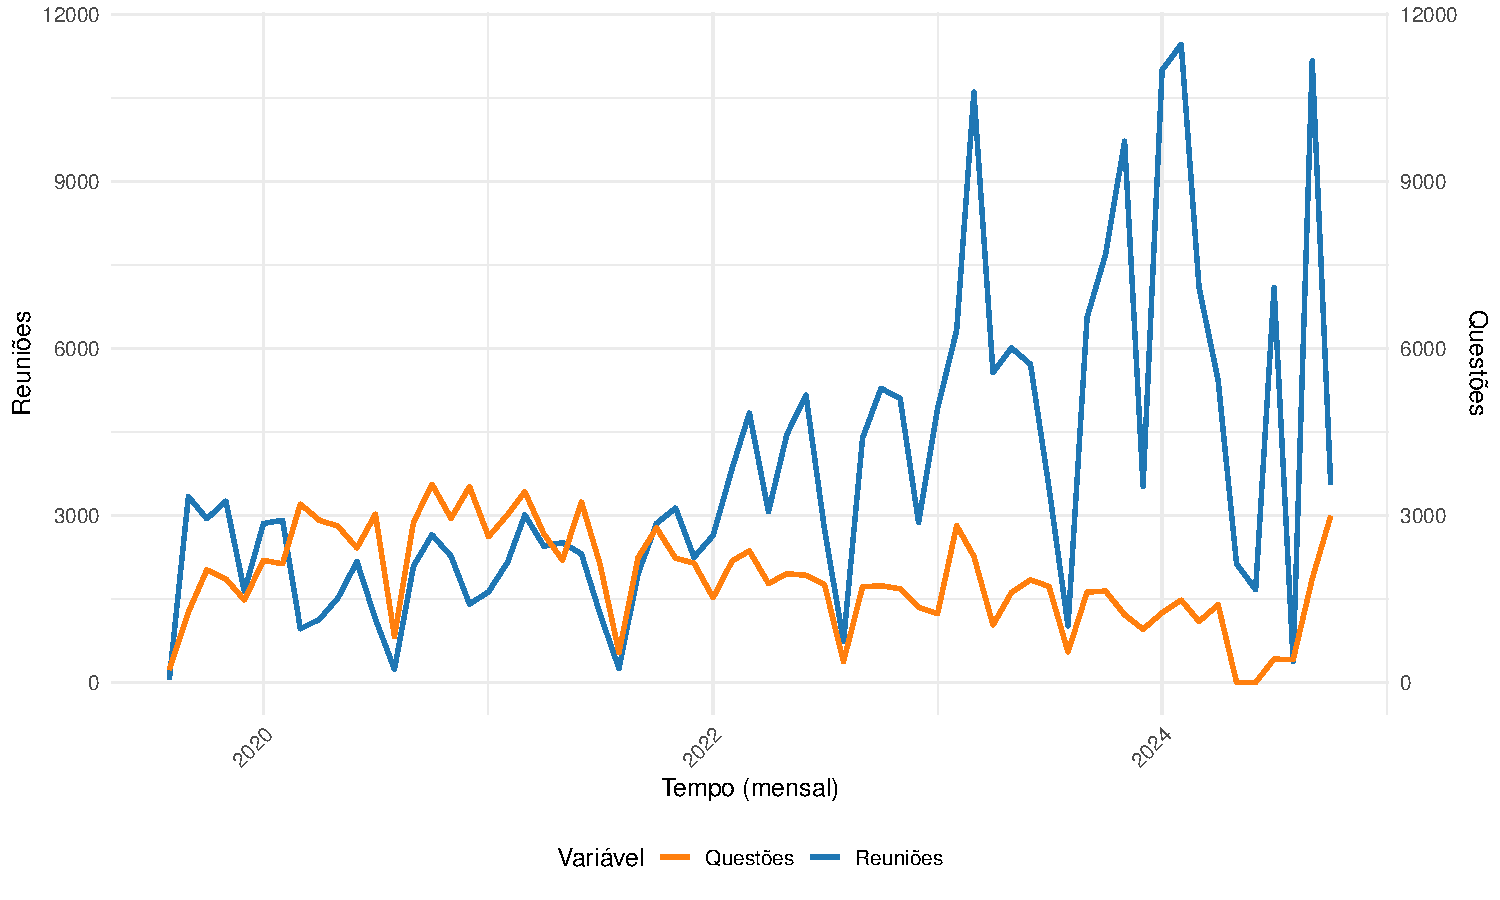
\includegraphics[width=0.9\textwidth]{figures/fig1_time_series_meetings_questions.pdf}
\caption{Evolução temporal da atividade parlamentar e de lobbying}
\end{figure}

\textbf{Padrões identificados:}
\begin{itemize}
\item Tendência crescente em ambas as variáveis
\item Sazonalidade relacionada ao calendário parlamentar
\item Picos de atividade coincidindo com discussões legislativas
\item Correlação contemporânea estável ao longo do tempo
\end{itemize}
\end{frame}

\begin{frame}{Distribuição do Tratamento}
\begin{columns}
\begin{column}{0.5\textwidth}
\begin{figure}
\centering
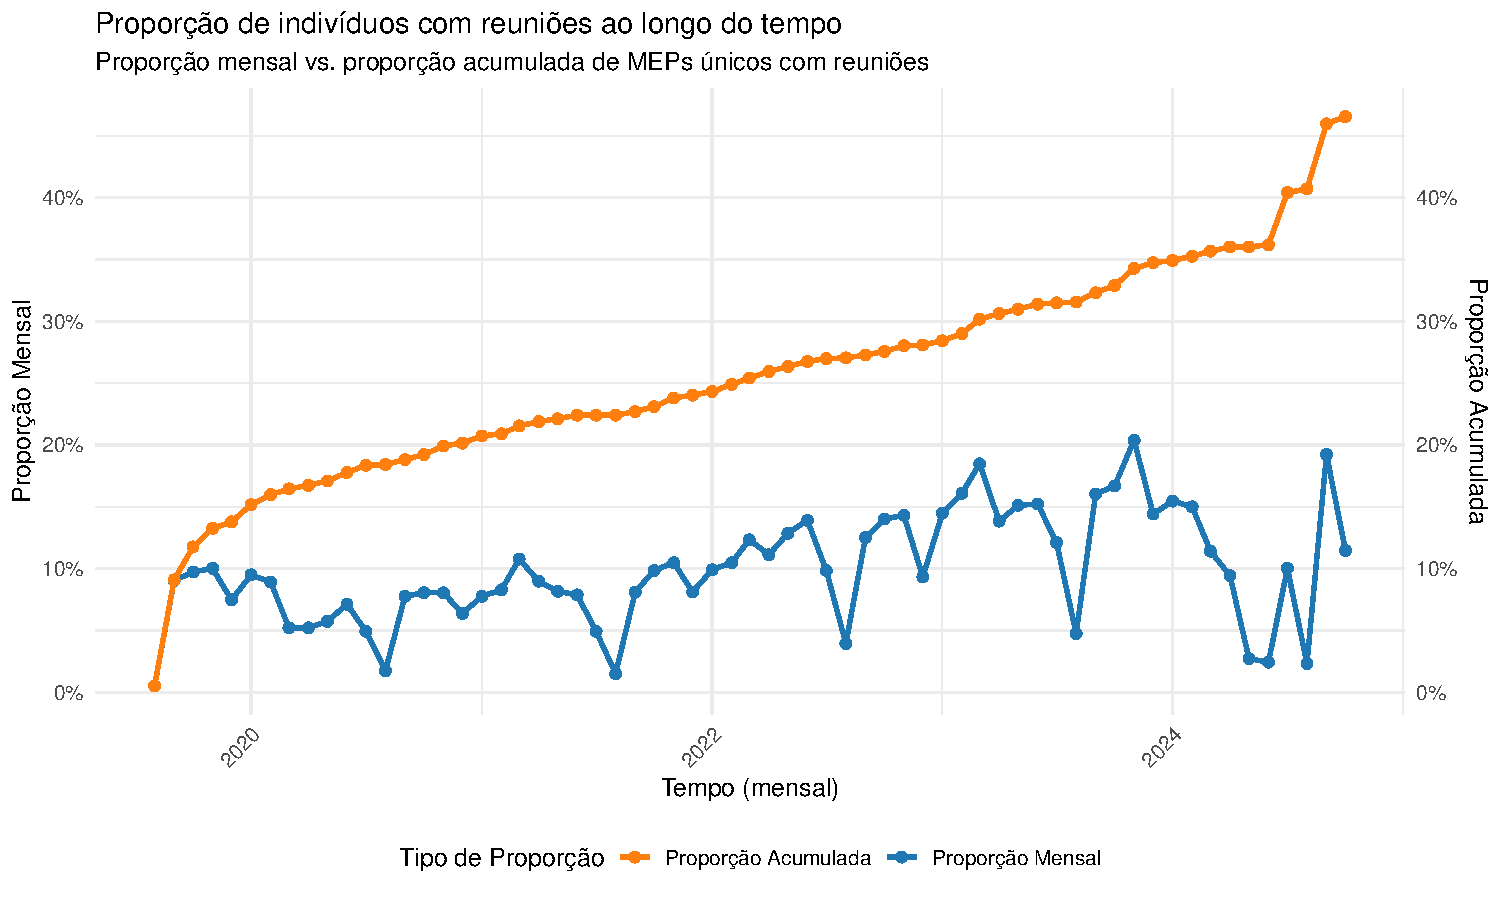
\includegraphics[width=\textwidth]{figures/fig2_proportion_meetings.pdf}
\caption{Proporção de MEPs com reuniões}
\end{figure}
\end{column}
\begin{column}{0.5\textwidth}
\begin{figure}
\centering
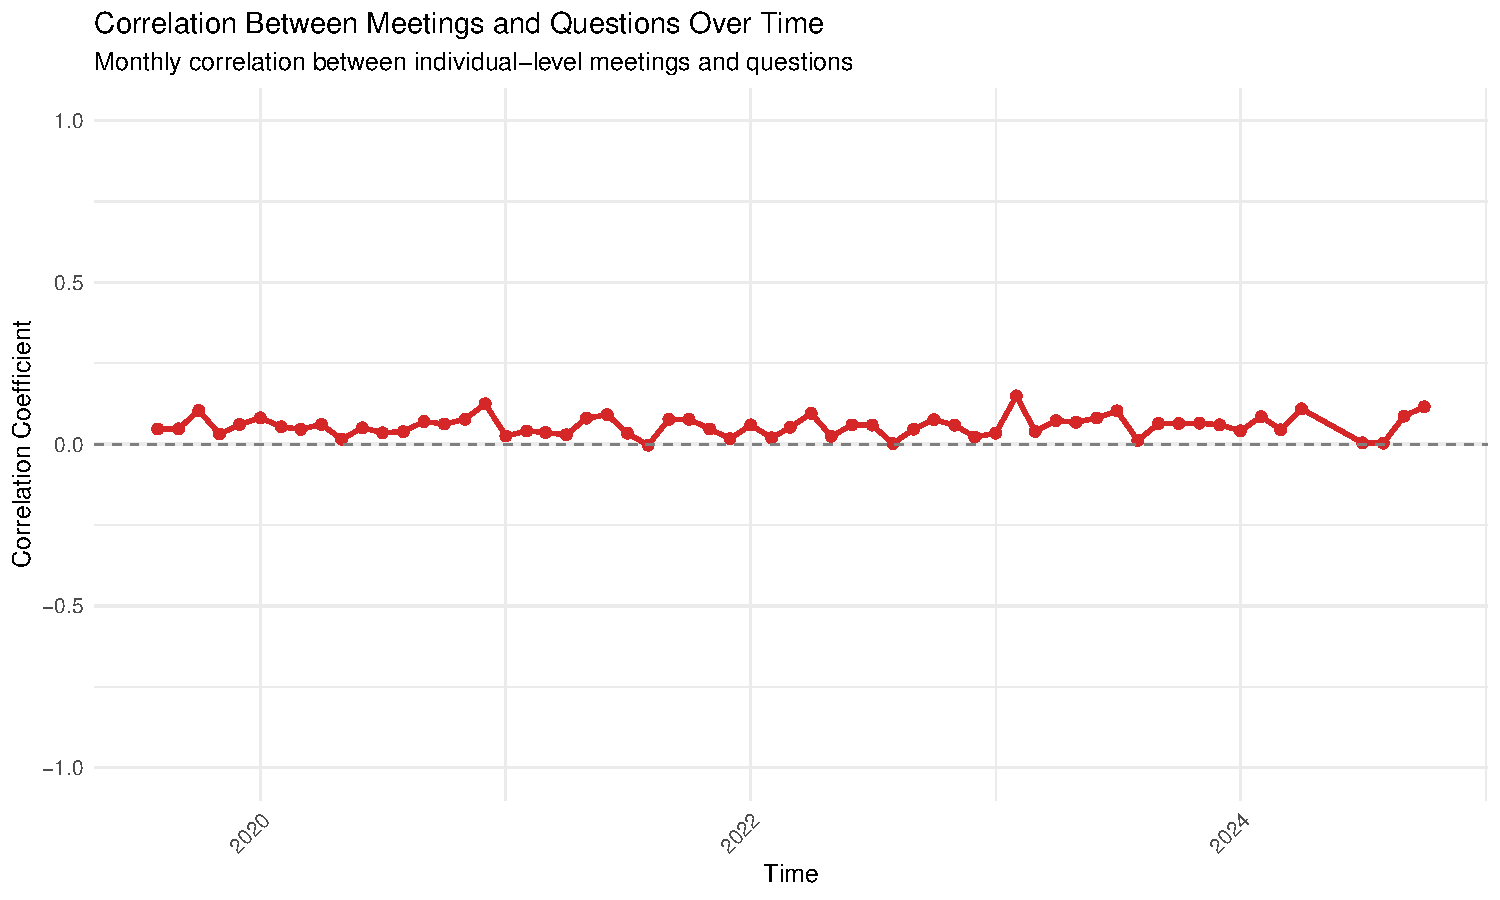
\includegraphics[width=\textwidth]{figures/fig3_correlation_meetings_questions.pdf}
\caption{Correlação temporal}
\end{figure}
\end{column}
\end{columns}
\end{frame}

\begin{frame}{Heterogeneidade por Domínio}
\begin{table}
\centering
\caption{Taxa de tratamento por domínio (\%)}
\begin{tabular}{lr}
\toprule
\textbf{Domínio} & \textbf{Taxa} \\
\midrule
Economia e Comércio & 45,5 \\
Tecnologia & 45,5 \\
Política Externa e Segurança & 45,2 \\
Infraestrutura e Indústria & 45,1 \\
Meio Ambiente e Clima & 44,9 \\
Saúde & 44,3 \\
Educação & 42,7 \\
Direitos Humanos & 41,7 \\
Agricultura & 40,9 \\
\bottomrule
\end{tabular}
\end{table}

\textbf{Padrão:} Domínios de regulação econômica apresentam maior atividade de lobbying
\end{frame}

\begin{frame}{Análise dos Lobistas}
\begin{columns}
\begin{column}{0.5\textwidth}
\textbf{Distribuição por Categoria:}
\begin{itemize}
\item \textbf{Business:} 33,7\%
\item \textbf{NGOs:} 32,8\%
\item \textbf{Outros:} 33,5\%
\end{itemize}

\textbf{Concentração Geográfica:}
\begin{itemize}
\item Bélgica: 18,2\%
\item Alemanha: 14,0\%
\item França: 9,3\%
\end{itemize}
\end{column}
\begin{column}{0.5\textwidth}
\begin{figure}
\centering
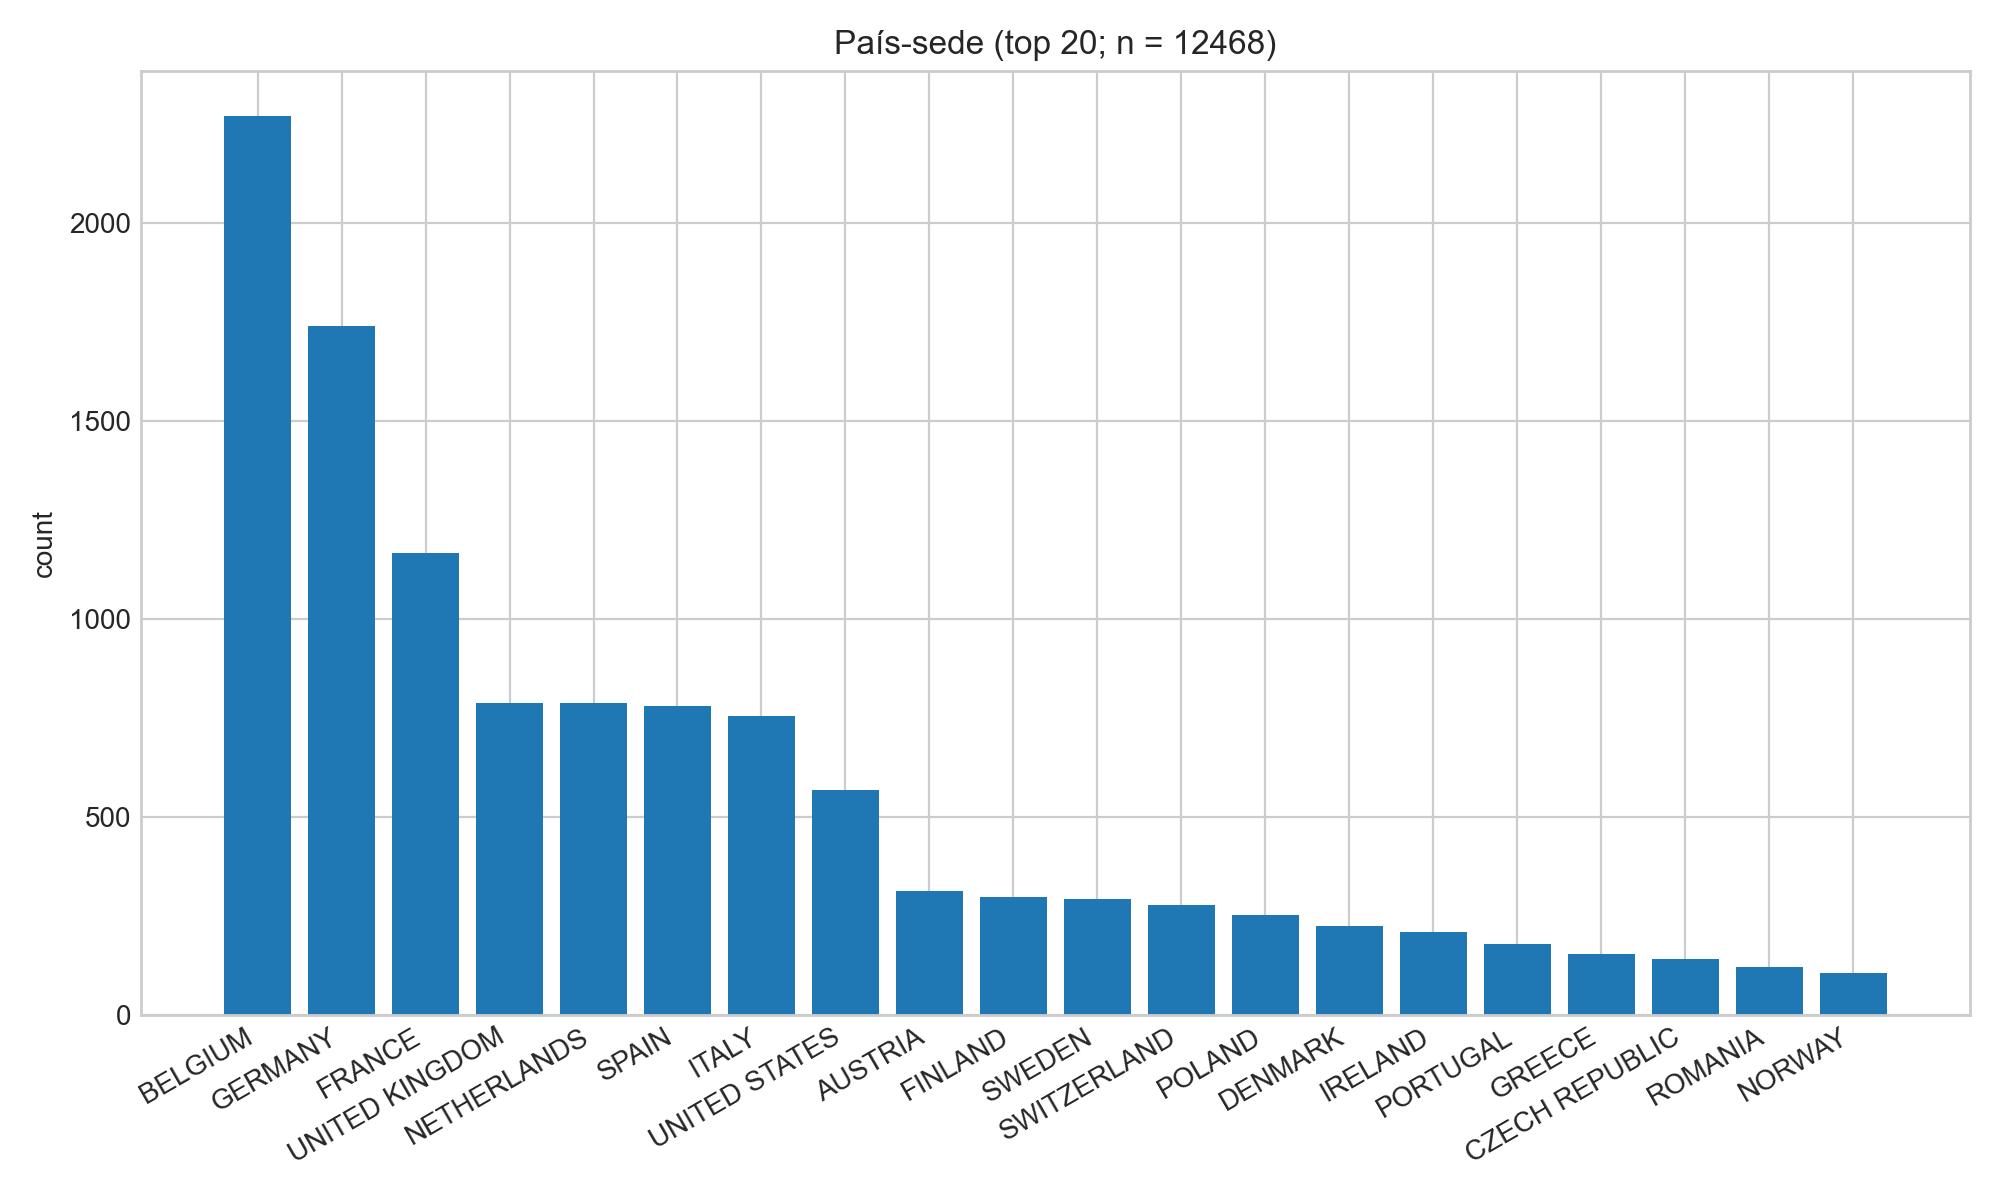
\includegraphics[width=\textwidth]{figures/country_distribution_top20.png}
\caption{Top 20 países-sede}
\end{figure}
\end{column}
\end{columns}
\end{frame}

% ========================================
% SEÇÃO 3: MODELAGEM ECONOMÉTRICA
% ========================================

\section{Modelagem Econométrica}

\begin{frame}{Escolha do Estimador: PPML}
\begin{block}{Justificativas para PPML}
\begin{enumerate}
\item \textbf{Natureza das variáveis:} Contagens com alta incidência de zeros
\item \textbf{Consistência:} Robusto a sobredispersão e heterocedasticidade
\item \textbf{Implementação:} Estável com efeitos fixos de alta dimensão
\end{enumerate}
\end{block}

\vspace{0.3cm}

\textbf{Forma funcional:} $\mathbb{E}[y\mid X] = \exp(X\beta)$

\textbf{Interpretação:} Coeficiente $\beta_k$ tem interpretação multiplicativa
\end{frame}

\begin{frame}{Estrutura de Efeitos Fixos}
\begin{block}{Estratégia de Identificação Causal}
\begin{itemize}
\item \textbf{$\mu_{id}$:} Efeitos fixos de membro (controla heterogeneidade não observada)
\item \textbf{$\mu_{ct}$:} Efeitos fixos país×tempo (controla choques comuns por país)
\item \textbf{$\mu_{pt}$:} Efeitos fixos partido×tempo (controla choques por partido)
\item \textbf{$\mu_{dt}$:} Efeitos fixos domínio×tempo (controla choques setoriais)
\end{itemize}
\end{block}

\vspace{0.3cm}

\textbf{Clustering:} Erros-padrão agrupados em domínio×tempo e membro
\end{frame}

\begin{frame}{Especificações do Modelo}
\begin{block}{Modelo Linear (Baseline)}
\begin{equation}
\text{questions}_{ijt} = \exp(\beta_1 \text{meetings}_{ijt} + \mathbf{X}_{ijt}\boldsymbol{\gamma} + \mu_{id} + \mu_{ct} + \mu_{pt} + \mu_{dt})
\end{equation}
\end{block}

\begin{block}{Modelo Quadrático (Retornos Marginais)}
\begin{equation}
\text{questions}_{ijt} = \exp(\beta_1 \text{meetings}_{ijt} + \beta_2 \text{meetings}_{ijt}^2 + \mathbf{X}_{ijt}\boldsymbol{\gamma} + \mu_{id} + \mu_{ct} + \mu_{pt} + \mu_{dt})
\end{equation}
\end{block}

\textbf{Controles:} Dummies de grupo político, país, comitês, delegações
\end{frame}

% ========================================
% SEÇÃO 4: RESULTADOS PRINCIPAIS
% ========================================

\section{Resultados Principais}

\begin{frame}{Resultados dos Modelos PPML}
\begin{table}
\centering
\caption{Estimativas principais: efeito de reuniões sobre perguntas}
\begin{tabularx}{\textwidth}{>{\raggedright\arraybackslash}p{.22\textwidth} >{\raggedright\arraybackslash}X >{\raggedright\arraybackslash}X}
    \toprule
      & PPML & PPML (Quad.) \\
    \midrule
    Reuni\~oes & 0,025*** (0,002) & 0,098*** (0,007) \\
    Reuni\~oes$^2$ &  & -0,004*** (0,001) \\
    \midrule
    Observa\c{c}\~oes & 600.237 & 600.237 \\
    Efeitos fixos & \multicolumn{2}{p{.72\textwidth}}{\raggedright pa\'is$\times$tempo; partido$\times$tempo; dom\'inio$\times$tempo} \\
    Cluster & \multicolumn{2}{p{.72\textwidth}}{\raggedright dom\'inio$\times$tempo; membro} \\
    \bottomrule
    \end{tabularx}
\end{table}

\textbf{Interpretação:} Coeficiente positivo e significativo indica associação positiva entre lobbying e atividade parlamentar
\end{frame}

\begin{frame}{Interpretação dos Resultados}
\begin{block}{Modelo Linear}
\begin{itemize}
\item \textbf{Efeito marginal:} $\frac{\partial \mathbb{E}[y]}{\partial x} = \beta_1 \exp(X\beta)$
\item \textbf{Interpretação:} Aumento de 1 reunião → variação de $100 \times (e^{0.066} - 1) = 6.8\%$ nas perguntas
\end{itemize}
\end{block}

\begin{block}{Modelo Quadrático}
\begin{itemize}
\item \textbf{Efeito marginal:} $\frac{\partial \mathbb{E}[y]}{\partial x} = (\beta_1 + 2\beta_2 x) \exp(X\beta)$
\item \textbf{Retornos decrescentes:} $\beta_2 < 0$ indica saturação de agenda
\item \textbf{Magnitude:} $\beta_2 = -0.002$ sugere retornos decrescentes pequenos
\end{itemize}
\end{block}
\end{frame}

\begin{frame}{Efeitos por Domínio}
\begin{figure}
\centering
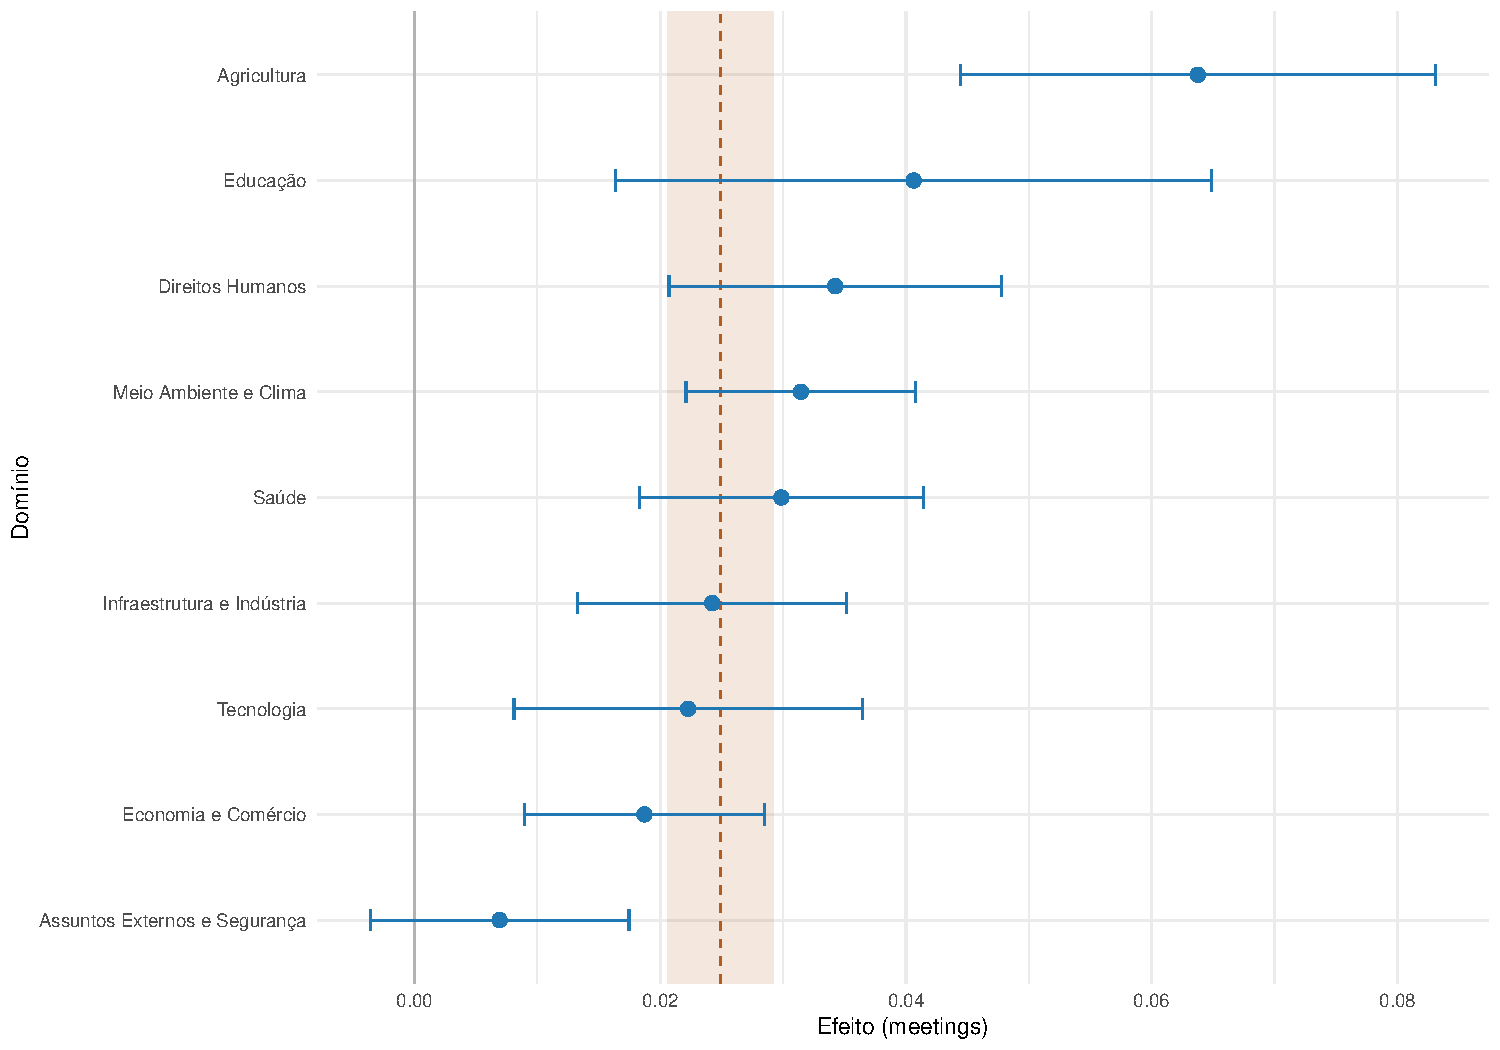
\includegraphics[width=0.9\textwidth]{figures/fig_coeff_domains.pdf}
\caption{Efeito do lobbying por domínio de política pública}
\end{figure}

\textbf{Resultado:} Efeito positivo consistente em todos os domínios, com variação na magnitude
\end{frame}

\begin{frame}{Efeitos por Tipo de Tratamento}
\begin{figure}
\centering
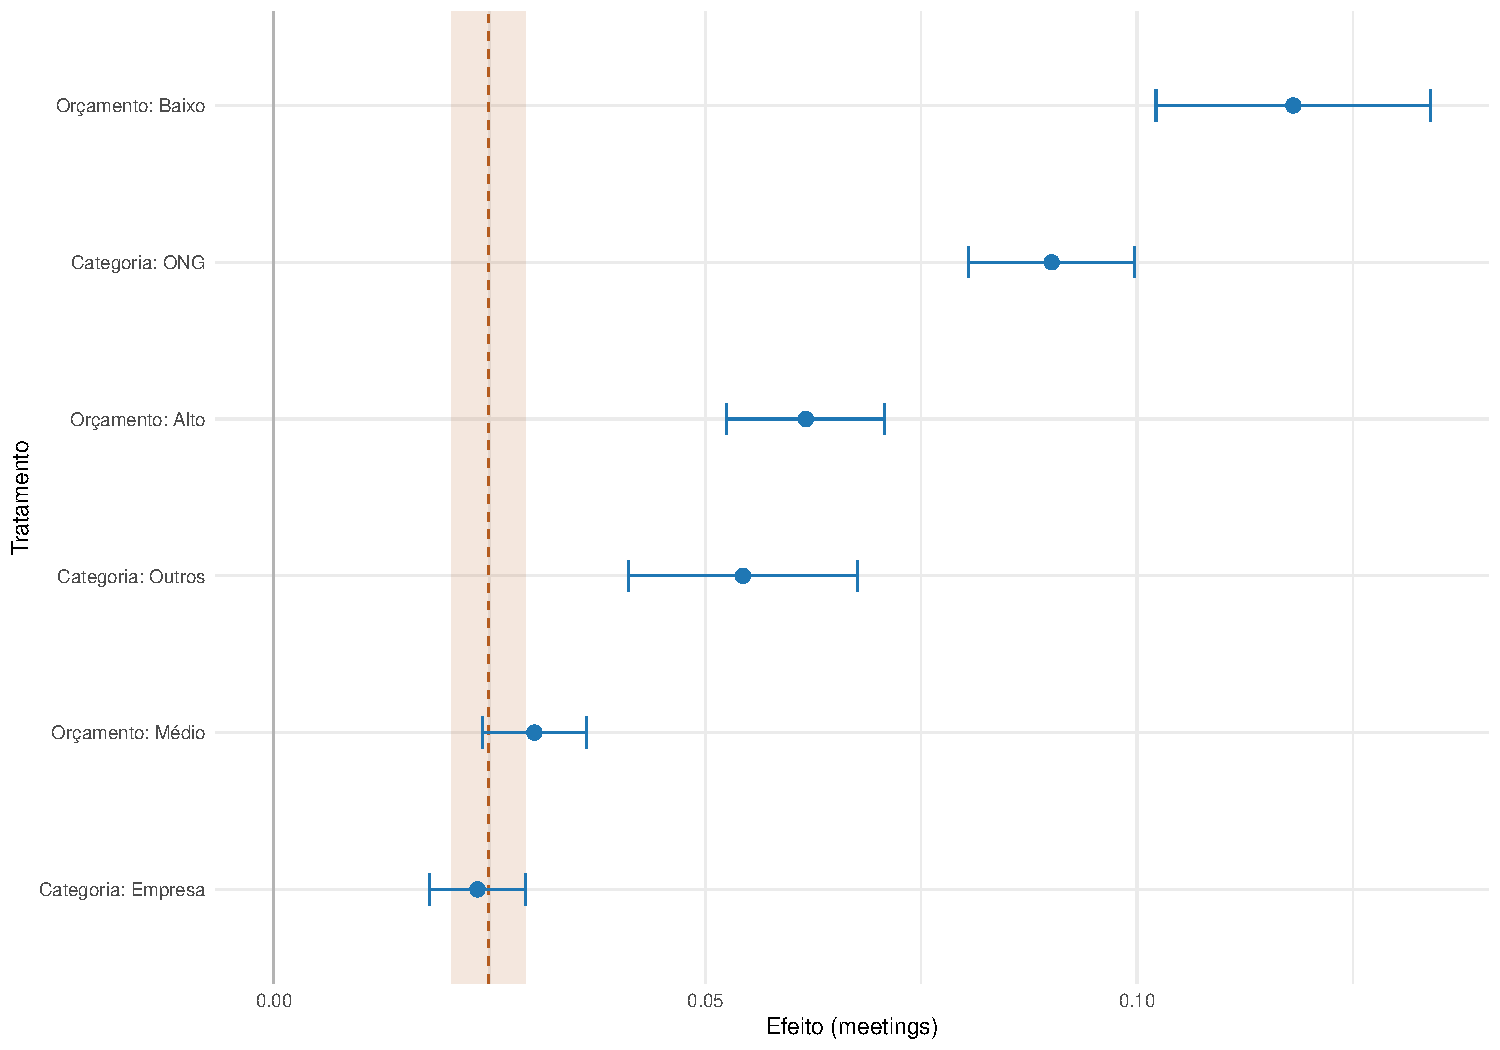
\includegraphics[width=0.9\textwidth]{figures/fig_coeff_treatments_overall.pdf}
\caption{Efeito do lobbying por categoria de organização}
\end{figure}

\textbf{Análise:} Heterogeneidade nos efeitos por tipo de organização lobista
\end{frame}

\begin{frame}{Curvas de Efeito}
\begin{columns}
\begin{column}{0.5\textwidth}
\begin{figure}
\centering
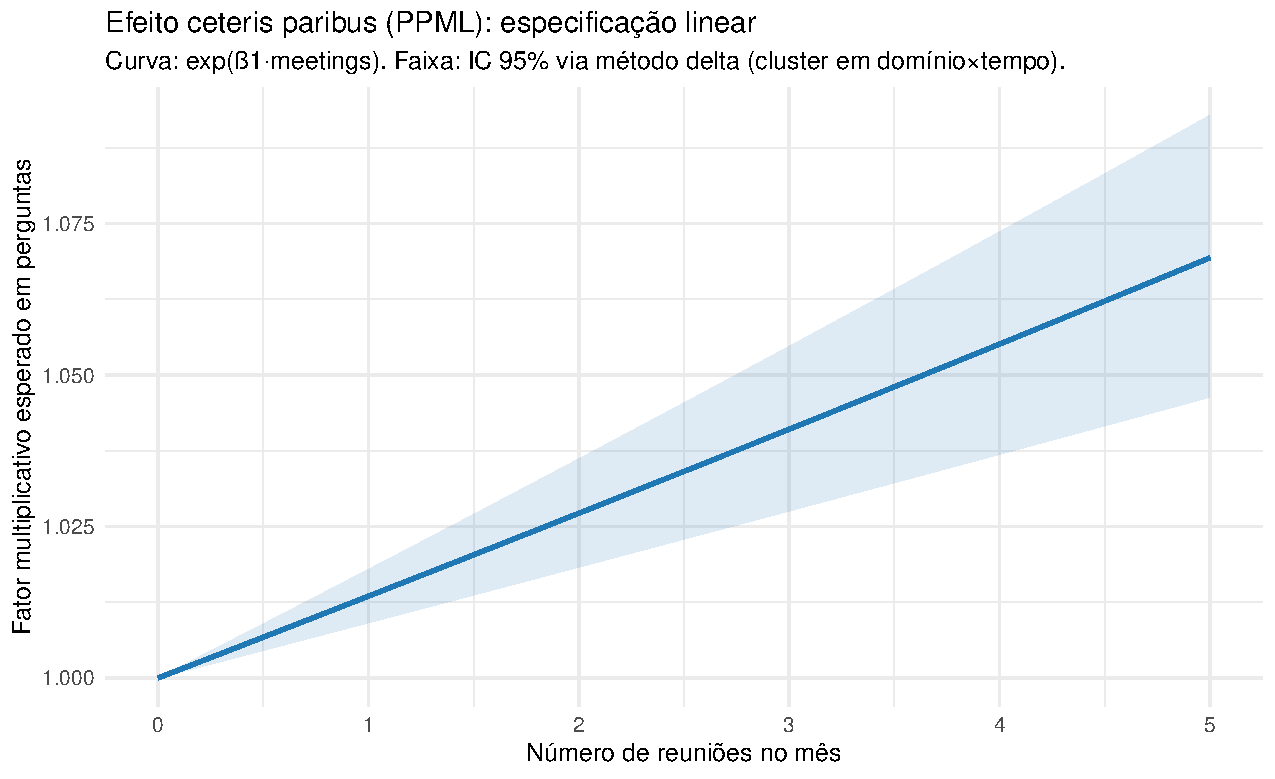
\includegraphics[width=\textwidth]{figures/fig8_effect_linear_ppml.pdf}
\caption{Especificação linear}
\end{figure}
\end{column}
\begin{column}{0.5\textwidth}
\begin{figure}
\centering
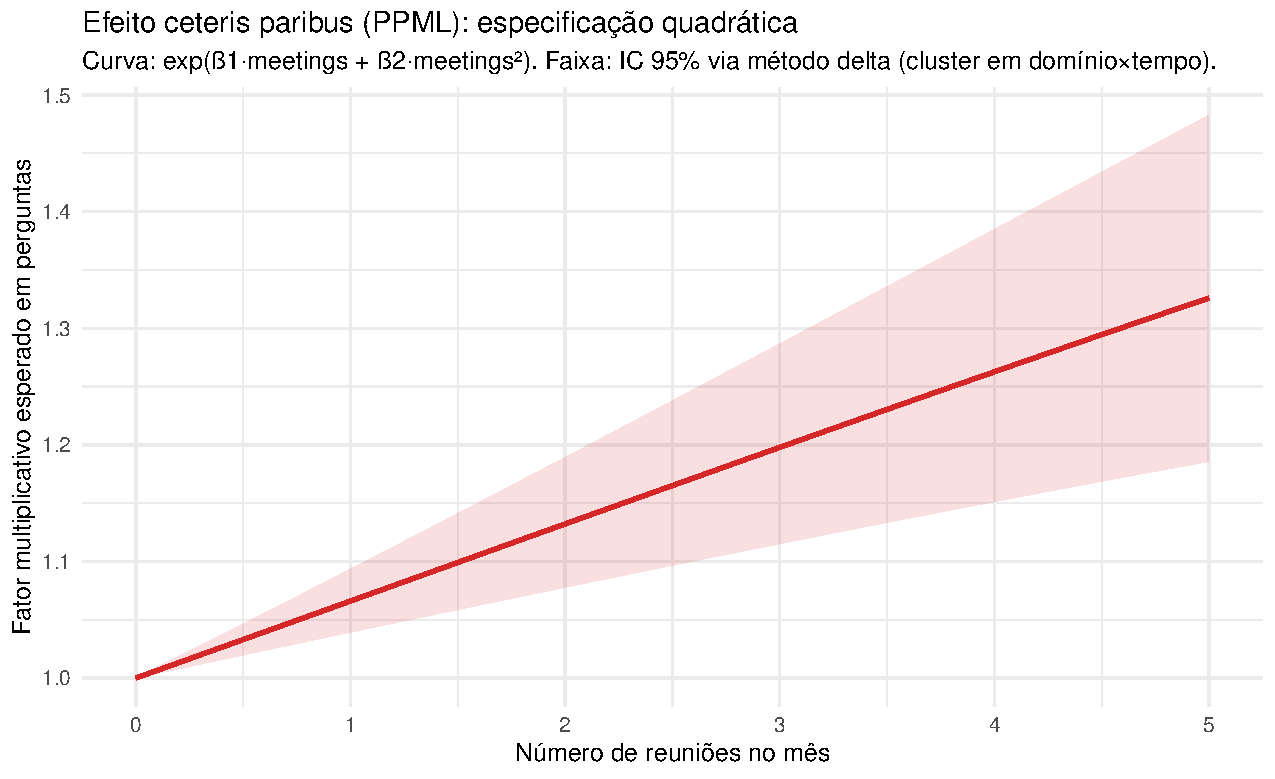
\includegraphics[width=\textwidth]{figures/fig9_effect_quadratic_ppml.pdf}
\caption{Especificação quadrática}
\end{figure}
\end{column}
\end{columns}

\textbf{Comparação:} Modelo quadrático captura retornos marginais decrescentes
\end{frame}

% ========================================
% SEÇÃO 5: ROBUSTEZ E IMPLICAÇÕES
% ========================================

\section{Robustez e Implicações}

\begin{frame}{Testes de Robustez}
\begin{block}{Especificações Alternativas}
\begin{itemize}
\item \textbf{Modelo linear vs. quadrático:} Resultados consistentes
\item \textbf{Diferentes tratamentos:} Categorias organizacionais, orçamento, experiência
\item \textbf{Análise por domínio:} Efeito positivo em todas as áreas temáticas
\item \textbf{Clustering robusto:} Erros-padrão em múltiplas dimensões
\end{itemize}
\end{block}

\vspace{0.3cm}

\textbf{Conclusão:} Resultados robustos a múltiplas especificações
\end{frame}

\begin{frame}{Implicações Teóricas e Políticas}
\begin{block}{Implicações Teóricas}
\begin{itemize}
\item \textbf{Confirmação da H1:} Lobbying aumenta atividade parlamentar
\item \textbf{Retornos decrescentes:} Eficácia diminui com intensidade excessiva
\item \textbf{Heterogeneidade setorial:} Efeitos variam por domínio de política
\end{itemize}
\end{block}

\begin{block}{Implicações Políticas}
\begin{itemize}
\item \textbf{Transparência:} Importância do registro de lobbying
\item \textbf{Regulação:} Necessidade de equilibrar acesso e influência
\item \textbf{Monitoramento:} Vigilância sobre concentração de esforços lobistas
\end{itemize}
\end{block}
\end{frame}

% ========================================
% SEÇÃO 6: LIMITAÇÕES E FUTURAS PESQUISAS
% ========================================

\section{Limitações e Futuras Pesquisas}

\begin{frame}{Limitações do Estudo}
\begin{block}{Desafios Metodológicos}
\begin{itemize}
\item \textbf{Endogeneidade:} Possível seleção não aleatória de reuniões
\item \textbf{Medição:} Captura apenas reuniões registradas oficialmente
\item \textbf{Defasagens:} Efeitos podem operar com timing diferente
\item \textbf{Generalização:} Resultados específicos ao contexto europeu
\end{itemize}
\end{block}

\vspace{0.3cm}

\textbf{Nota:} Efeitos fixos e clustering mitigam mas não eliminam todas as preocupações
\end{frame}

\begin{frame}{Direções para Pesquisa Futura}
\begin{block}{Extensões Metodológicas}
\begin{itemize}
\item \textbf{Instrumentação:} Identificação de choques exógenos no lobbying
\item \textbf{Análise de defasagens:} Estrutura temporal dos efeitos
\item \textbf{Mecanismos:} Canais específicos de influência
\end{itemize}
\end{block}

\begin{block}{Extensões Substantivas}
\begin{itemize}
\item \textbf{Outcomes:} Votação, relatórios, emendas
\item \textbf{Contextos:} Outros parlamentos nacionais
\item \textbf{Períodos:} Análise de longo prazo e mudanças institucionais
\end{itemize}
\end{block}
\end{frame}

% ========================================
% SEÇÃO 7: CONCLUSÕES
% ========================================

\section{Conclusões}

\begin{frame}{Principais Conclusões}
\begin{block}{Evidências Empíricas}
\begin{enumerate}
\item \textbf{Associação positiva:} Lobbying aumenta atividade parlamentar de fiscalização
\item \textbf{Retornos decrescentes:} Efeito marginal diminui com intensidade
\item \textbf{Robustez:} Resultados consistentes em múltiplas especificações
\item \textbf{Heterogeneidade:} Efeitos variam por domínio e tipo de organização
\end{enumerate}
\end{block}

\vspace{0.3cm}

\textbf{Contribuição:} Evidência quantitativa robusta sobre efeitos do lobbying no Parlamento Europeu
\end{frame}

\begin{frame}{Implicações para a Literatura}
\begin{block}{Contribuições Principais}
\begin{itemize}
\item \textbf{Metodológica:} Aplicação de PPML com efeitos fixos de alta dimensão
\item \textbf{Empírica:} Primeira análise sistemática do lobbying europeu
\item \textbf{Teórica:} Confirmação de mecanismos de influência política
\item \textbf{Política:} Base para discussões sobre regulação do lobbying
\end{itemize}
\end{block}

\vspace{0.3cm}

\textbf{Relevância:} Estudo pioneiro que abre caminho para pesquisas futuras
\end{frame}

% Slide final
\begin{frame}
\begin{center}
\Large \textbf{Obrigado!}

\vspace{1cm}
\textbf{Perguntas e Discussão}

\vspace{1cm}
\small
\textit{Efeitos do Lobbying na Atividade Parlamentar: \\ Modelagem PPML e Análise Causal}
\end{center}
\end{frame}

\end{document}
